\begin{figure}
	\begin{center}
	\tikzsetnextfilename{monotone_fkt_riemann_intbar}
		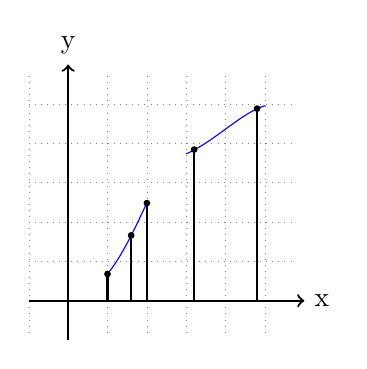
\begin{tikzpicture}
			\draw[dotted, very thin, gray, step = 0.5] (0,-0.9) grid (3.4,2.4);
			
			\draw[->, thick, black](0,-0.5) -- (3.5,-0.5) node[right]{x};
			\draw[->, thick, black](0.5, -1) -- (0.5, 2.5) node[above]{y};
			\draw[blue, domain = 1 :1.5, samples = 1000]  
				plot(\x, {\x * \x * sin(\x r) - \x });
			
			\draw[blue, domain = 2 :3, samples = 1000]  
				plot(\x, {\x * \x * sin(0.5*\x r) - \x*\x + 2});	
			
			\draw[fill=black](1,-0.16)circle(1pt);
			\draw[fill = black](1.3,0.33) circle(1pt);
			\draw[fill = black] (1.5, 0.74) circle(1pt);
			\draw[thick, black](1,-0.5) -- (1, -0.16);
			\draw[thick, black](1.3,-0.5) --(1.3, 0.33);
			\draw[thick, black](1.5,-0.5) --(1.5, 0.74);
			
			\draw[fill = black](2.1,1.42) circle (1pt);
			\draw[fill = black](2.9,1.94) circle(1pt);
			\draw[thick, black](2.1, -0.5) -- (2.1, 1.42);
			\draw[thick, black](2.9, -0.5) -- (2.9, 1.94);
		
		\end{tikzpicture}
	\end{center}
	\caption{Monotone Funktion}
	\label{fig:Monotone_Funktion_Riemannint}
\end{figure}